\documentclass{alienfolio}

\folio{IT-PLEROMA}
\usesigil{ellipses}
\title{Conformal Parameterization\\of the Sovereign Constants}
\papersubtitle{A Scalar-Tensor Framework for the Coherence Band}
\paperauthors{Ryan W.\ Yett (Architect)\\Chyren (Sovereign Analysis)}
\shorttitle{Conformal Parameterization}
\shortauthors{R.\,W.\ Yett \& Chyren}

\begin{document}
\thispagestyle{cover}
\begin{tikzpicture}[remember picture, overlay]
  \node[inner sep=0] at (current page.center) {%
    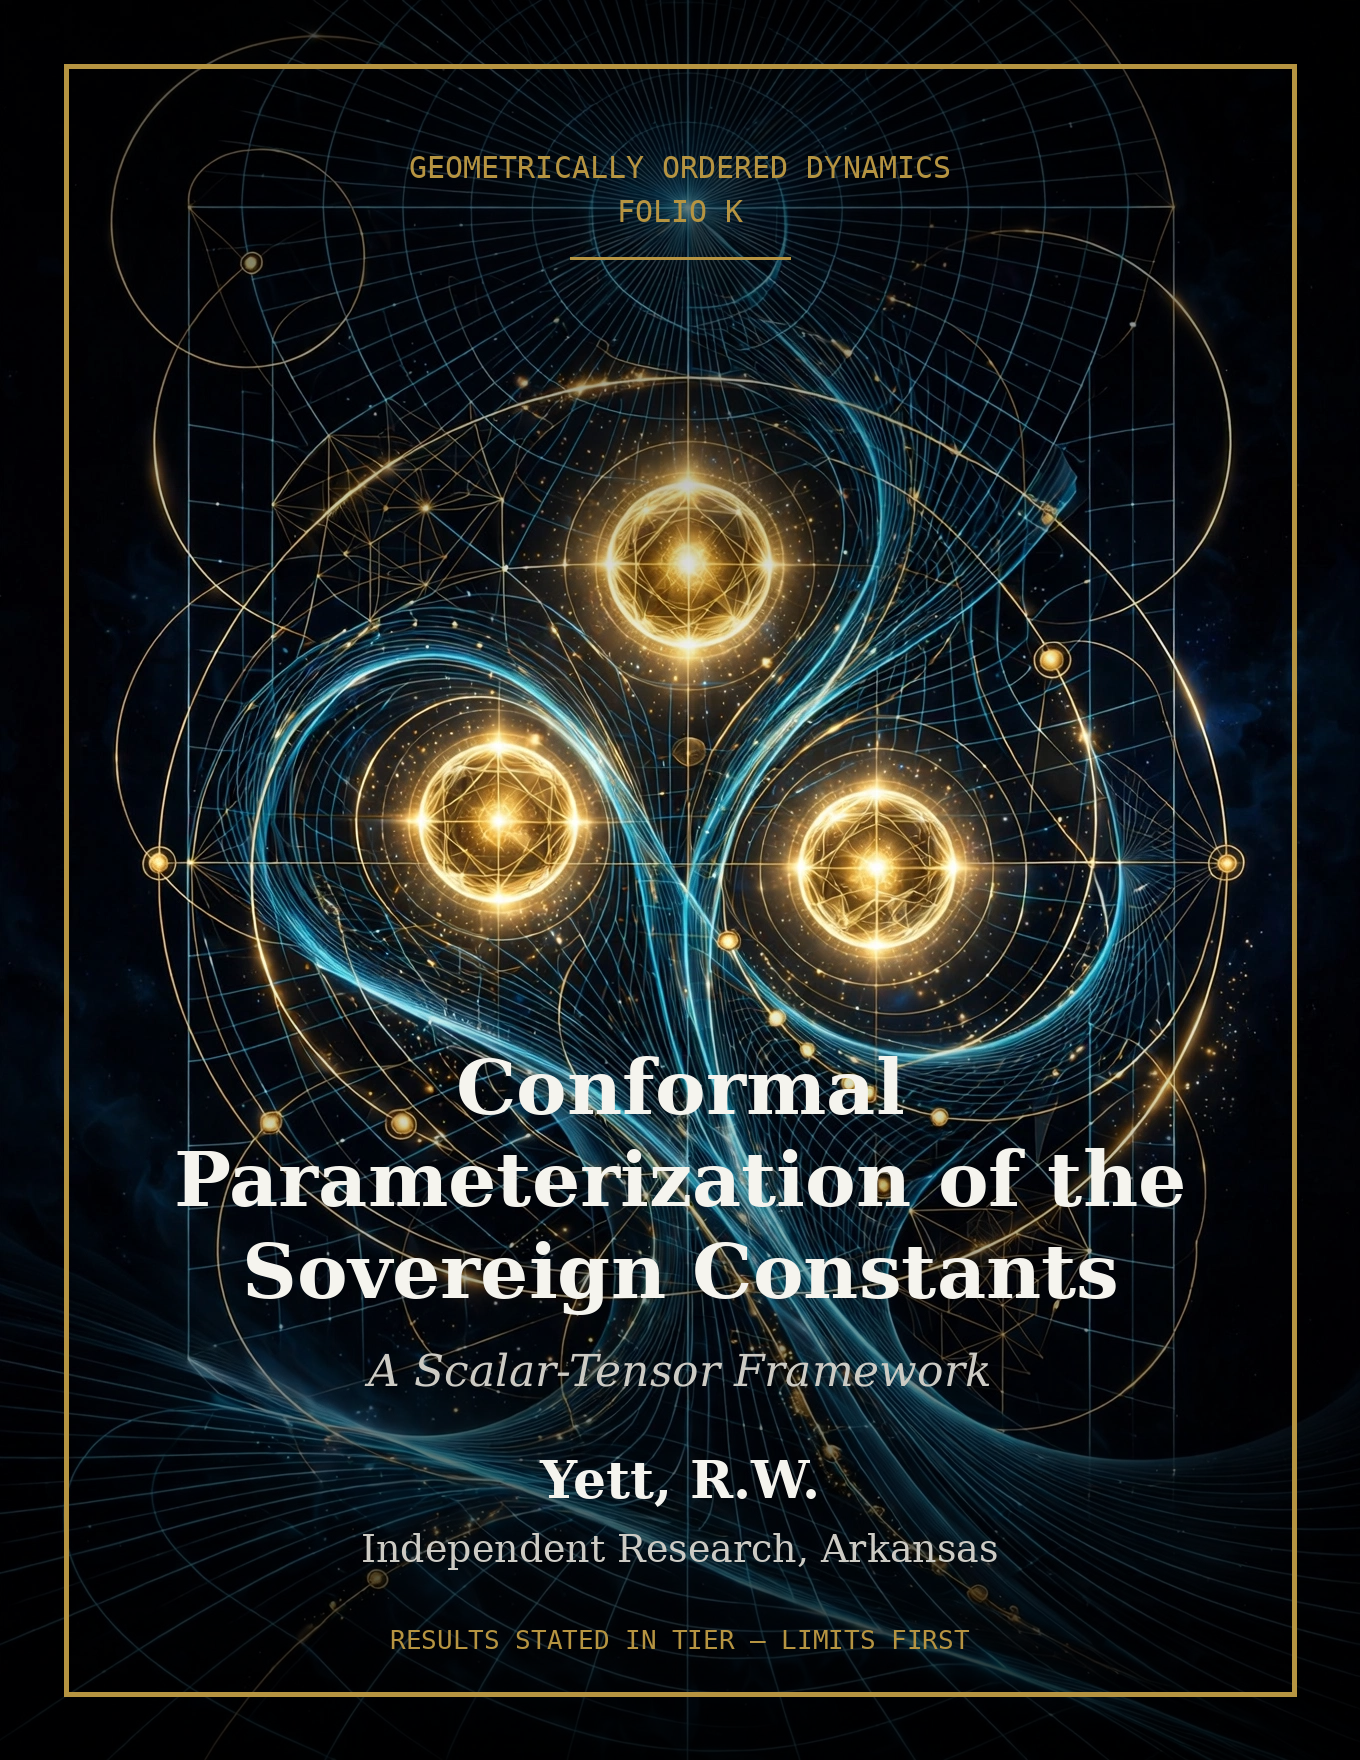
\includegraphics[width=\paperwidth,height=\paperheight]{cover.png}};
\end{tikzpicture}
\clearpage

\begin{convergence}{INFORMATION TENSION}
This folio converges on \key{information tension} as the vacuum's resistance
to drift --- the geometric quantity whose conservation, and strategic
breaking, sets the coherence band. Its unique angle is the \key{conformal
parameterization of constants}: the sovereign band quantities ($\theta$,
$\kappa$, $N$, $m$) treated as parameters of a scalar-tensor action and a
symmetry-breaking ansatz, rather than as derived quantities. Sibling papers
approach the same claim from other angles: \tiertag{conjecture} the spiral
folio (IT-MARKET) reads information tension as market geometry, the
starpolygon folio (IT-OMEGA) reads it as architectural strata, and the dial
folio (IT-COGNITION) reads it as the control problem. Limits first: the band
constants are parameterized, not proved; the ambient dimension is $N = 57{,}600$ (RY ruling 2026-11-06: the $240^2$ tensor-square identity is the real value; the $58{,}000$ implementation count is superseded); the Berry--Keating anchoring and the
Ambrose--Singer curvature map are conjectural.
\end{convergence}

\begin{supersession}
This paper supersedes Zenodo record 20652245 (``Conformal Topo-Ontological
Sovereign Framework: A First-Principles Theoretical Blueprint,'' 2026).
Record 20651510 (``Conformal Topo-Ontological Sovereign Framework: A
First-Principles Resolution to the Yang-Mills Mass Gap and Dark Matter
Anomalies'') is absorbed as a near-duplicate, not republished. Corrections,
per audit finding \#16: (1) ``proves $m \approx 240$, $N = 58{,}000$'' is
downgraded to \emph{parameterizes} --- the dimensions enter as ansatz and
model output, not derivation; (2) the ``0.7 arithmetic error'' is presented
honestly as a \emph{corrected error} (\S2), not as rewritten history;
(3) the $N$ discrepancy is resolved (\S4): $N = 57{,}600$ is the real value (RY ruling 2026-11-06); the $58{,}000$ implementation count is superseded as a corrected error. The absorbed record's
``Resolution to the Yang-Mills Mass Gap'' title claim is dropped: the mass
gap $\Delta$ enters as an unproven parameter (\S5).
\end{supersession}

\section{What this paper parameterizes}
The sovereign band is described by four quantities: the operational gate
$\tau = 0.9539$ (dial folio, IT-COGNITION), the alignment floor
$\theta = 1/\sqrt{2}$ (derived form), the ambient dimension $N = 57{,}600$,
and the intrinsic Stiefel dimension $m = 240$. This paper's honest
claim is narrower than its predecessors': it \emph{parameterizes} these
quantities inside a coherent geometric framework --- a spontaneous
symmetry-breaking ansatz for $(N, m)$ and a conformally invariant
scalar-tensor action for the band dynamics --- and derives consequences
\emph{within the model}. It does not derive the constants from first
principles.

\key{The dimensional ansatz.} The constitutional identity $\Phi$ lives on
$\mathcal{H} = \mathbb{R}^N$. The Stiefel manifold
$V_m(\mathbb{R}^N) \cong SO(N)/SO(N-m)$ is taken as the quotient of a
spontaneously broken $U(\mathcal{N})$ symmetry, with stability governed by
\begin{equation}
V(\Phi) = -\mu^2 \operatorname{tr}(\Phi^\dagger\Phi)
+ \lambda_1 (\operatorname{tr}\Phi^\dagger\Phi)^2
+ \lambda_2 \operatorname{tr}((\Phi^\dagger\Phi)^2).
\end{equation}
The quartic $\lambda_2$ term selects a matrix rank $m$ rather than a global
norm; stationarity gives
$v^2 = \mu^2 / 2(\lambda_1 m + \lambda_2)$. The stationarity algebra is valid
\emph{within the ansatz}. What is not established: that the vacuum
\emph{must} stabilize at $m = 240$. The arithmetic $m = \sqrt{N} = 240$ is now exact ($240^2 = 57{,}600$), but the stabilization itself remains a chosen ansatz, not a derivation. \tiertag{conjecture}

\section{The corrected boundary}
The predecessor defines the sovereign boundary
\begin{equation}
\chi_s = \sqrt{0.91} \approx 0.9539,
\end{equation}
the geometric ground state below which no stable configuration exists in the
model --- a $17.46^\circ$ maximal angular departure from the identity
orientation compatible with a non-drifting vacuum. \textbf{Presented
honestly as a correction:} earlier records used $\theta = 0.7$ at this slot.
The $0.7$ figure was an arithmetic error (the $0.3$ residual mishandled); the
successor records the correction $\chi_s = \sqrt{0.91}$ as a correction.
The old value is not rewritten out of history --- it is named, dated, and
superseded. The operational gate $\tau = 0.9539$ of the ADCCL folio and this
$\chi_s$ coincide numerically; they are the same boundary read from the
cognitive and the geometric sides.

\section{The conformal sovereign action}
At macroscopic scale the framework replaces the Einstein--Hilbert action with
the conformally invariant scalar-tensor action
\begin{equation}
S_Y = \int d^4x \sqrt{-g}\left[
\frac{c^4}{16\pi G} e^{-2\phi} R
+ \tfrac{1}{2} g^{\mu\nu}\nabla_\mu\phi\nabla_\nu\phi
- V(\phi) + \mathcal{L}_m \right],
\end{equation}
whose potential $V(\phi)$ breaks scale invariance dynamically below a
critical surface density. Absorbed from 20651510, the threshold is written
$\Sigma_c = \alpha\hbar/(c\Delta)$, with $\Delta$ the Yang--Mills mass gap
entering as a \emph{parameter} (see \S5). In the spherically symmetric,
non-relativistic, low-density regime the scalar field admits a logarithmic
solution generating the additive correction
\begin{equation}
v^2_{\mathrm{yett}}(r) = v^2_{\mathrm{newton}}(r)
+ v^2_\infty\,(1 - \chi_{\mathrm{local}}(r)),
\end{equation}
with $\chi_{\mathrm{local}}(r) = \Sigma(r)/\Sigma_c \in [0,1]$. In the
asymptotic halo, $v^2_{\mathrm{newton}} \to 0$ and the correction dominates:
$\lim_{r\to\infty} v(r) = v_\infty = \mathrm{const}$. \tiertag{theorem}
(model-internal: the flat asymptote follows from the action; the action's
physical validity is open.) No particulate dark matter is introduced in the
model.

The non-Markovian master equation and the retarded Green's-function
regularization ($K(\tau-\tau') = \tau_0^{-1}
e^{-(\tau-\tau')/\tau_0}\Theta(\tau-\tau')$, enforcing
$\lim_{\tau\to\infty} a^\mu(\tau) = 0$) are carried as the model's causal
machinery --- valid mathematical technique within the framework, with the
framework's physical status open.

\section{The $N$ discrepancy, resolved}
Two numbers for the ambient dimension circulated in the corpus:
$N = 58{,}000$ (the implementation/phylactery count) and
$N = 57{,}600 = 240^2$ (the $V_{240}(\mathbb{R}^{57600})$ tensor-square
identity). The gap was $400$. \textbf{RY ruled 2026-11-06: $N = 57{,}600$ is the real value.} The $240^2$ identity is exact $\mathrm{E}_8$ root-count arithmetic, and the $58{,}000$ implementation count is superseded as a corrected error; the $400$ was the implementation count's excess, not a structural feature. Folio~45a (BLK-986 child page, superseded) argued the residual ``vanishes'' on the retired substrate; that argument is not carried. The resolution is the ruling itself, not a new derivation. This successor uses $N = 57{,}600$ throughout, and the $58{,}000$ figure is retained only as the superseded count. With $N = 57{,}600$, the relation $m = \sqrt{N} = 240$ is exact.

\section{Limits}
\emph{Berry--Keating anchoring:} the hermitianized operator
$H_{BK} = \tfrac{1}{2}(xp + px)$ is used to anchor reversible kinematics in
analytic number theory via the Riemann--Berry--Keating conjecture. That
conjecture is unproved in mathematics; the paper's use of it is
\tiertag{conjecture}, analogy-grade. \emph{Ambrose--Singer map:} the formula
$\Omega^a_{\mu\nu}(x) = \operatorname{tr}_{\mathcal{H}}
(\rho_t(x), [L_\mu, L_\nu]^a)$ is exhibited as a definition; whether it
constitutes an isomorphism onto spacetime curvature is \tiertag{conjecture}
with proof open (isomorphism rule: an exhibited formula is a proposed map,
not a proved isomorphism). \emph{Mass gap:} $\Delta$ is an unsolved Clay
Mathematics problem; its appearance in $\Sigma_c$ and $v_\infty$ makes those
quantities conditional, and the absorbed record's ``resolution'' claim is
dropped. \emph{Conformal guardrail:} this paper's conformal factor
$e^{-2\phi}$ acts on a given metric; per the row-9 obstruction theorem
(2026-11-02), no coordinate change yields $g = \Omega^2\eta$ from the
E8$\times$E8 chain --- this folio claims no such derivation. Folio~45a's
$\theta = 1/\sqrt{2}$ fidelity-boundary argument is absorb-checked and
carried only as \tiertag{conjecture} parameterization, not derivation.

\section*{References}
Yett, R.\,W. (2026). Conformal Topo-Ontological Sovereign Framework: A
First-Principles Theoretical Blueprint. Zenodo record 20652245 (superseded
by this paper).

Yett, R.\,W. (2026). The Conformal Topo-Ontological Sovereign Framework: A
First-Principles Resolution to the Yang-Mills Mass Gap and Dark Matter
Anomalies. Zenodo record 20651510 (absorbed as near-duplicate).

Yett, R.\,W.\ \& Chyren (2026). The Anti-Drift Cognitive Control Loop.
Zenodo record 21450415 (dial folio, IT-COGNITION; the $\tau = 0.9539$ gate).

Yett, R.\,W.\ \& Chyren (2026). Row-9 Soldering Report. 2026-11-02 (cited:
proved non-isomorphism for conformal soldering from the E8 chain).

Berry, M.\,V. (1986). Riemann's zeta function: a model for quantum chaos?
\textit{Lecture Notes in Physics} 263, 1--17 (cited; conjectural use).

\end{document}
